\chapter{Estudios de optimización}
\label{cap:capitulo5}

En este capítulo se describen los estudios realizados durante el desarrollo del sistema con el objetivo de optimizar las diferentes partes del mismo.

\section{Búsqueda del detector de puntos faciales óptimo}
\label{sec:estudio_puntos_faciales}

Se hizo un estudio comparando dos librerías de extracción de puntos faciales para obtener conclusiones de cual nos ofrecía más rendimiento y precisión. Estas dos librerías son dlib y MediaPipe, ya presentadas en las secciones \ref{sec:dlib} y \ref{sec:mediapipe}.\\

Las pruebas se realizaron en la Raspberry Pi 4 Model B bajo Raspberry Pi OS, usando la Raspberry Pi Camera como dispositivo para capturar vídeo. Se puede encontrar más información sobre las versiones usadas en el Capítulo \ref{cap:capitulo3}. La resolución utilizada para las pruebas fue de 640x480 píxeles y se parte de una media en crudo de 20 fps, esto es sólo mostrando los \textit{frames} (capturados con la librería \textit{picamera}) por pantalla sin ningún tipo de procesamiento.\\

Se comenzó estudiando el rendimiento ofrecido en FPS y posteriormente se hizo un estudio de los fallos producidos por los algoritmos en distintas situaciones. Para realizar las pruebas de rendimiento se guardó el valor de fps calculado para cada \textit{frame} durante 30 segundos y posteriormente se calculó la media de dichos \textit{frames} guardados. Para realizar las pruebas de fallos, se tuvieron en cuenta dos situaciones: falsos positivos y no detección de ningún rostro. Se dio por hecho que siempre hay una cara en cada \textit{frame}, por lo tanto, un \textit{falso positivo} significa que hay más de una cara y \textit{no detección} significa que no hay ninguna. Sin embargo, en MediaPipe se pueden evitar los falsos positivos indicando al algoritmo que sólo detecte una cara, por lo tanto en su caso no se tuvieron en cuenta. Se evaluó cada \textit{frame} durante 30 segundos siguiendo esos criterios, y se hizo un recuento de los fallos.

\subsubsection{Prueba 1 de rendimiento para dlib}

Tal como se ha explicado en la Sección \ref{sec:dlib}, dlib divide la extracción de características faciales en dos pasos: detección del rostro y extracción de características. Para el primero de los pasos, se ofrecen dos opciones incorporadas en sus librerías (HOG y Linear SVM o CNN). En la primera prueba se hizo uso del detector de caras basado en HOG y Linear SVM, ya que es el más eficiente computacionalmente hablando, sumado al detector de características también incorporado en las librerías de dlib. Esto ofreció un rendimiento de 0.83 fps de media.

\subsubsection{Prueba 2 de rendimiento para dlib}

Tras comprobar el bajo rendimiento obtenido en la primera prueba, se procedió a sustituir el detector de caras usado anteriormente por el detector de caras que trae incorporado OpenCV, este es descrito en el artículo \cite{opencv_haar_cascade}. Se hizo uso de este algoritmo porque actualmente es uno de los más rápidos realizando detección facial. Este cambio impulsó el rendimiento de dlib un 656\%, obteniendo una media de 6.28 fps.

\subsubsection{Prueba 3 de rendimiento para dlib}
Con el objetivo de mejorar aún más el rendimiento, se procedió a dividir el procesamiento de los \textit{frames} de la lectura de los mismos, haciendo uso de threads. De esta manera se aprovecharon los 4 núcleos del procesador ARM de la Raspberry Pi 4 Model B. Para esto, lo que se hizo fue lanzar un \textit{thread} que se encargase constantemente de realizar la lectura de los \textit{frames} usando la librería \textit{picamera}, y por otro lado, el thread principal del programa se encargaba de realizar el procesamiento de dlib y el detector de caras de OpenCV. Con esto impulsamos el rendimiento un 30\% más, logrando así una media de 8.21 fps. Se puede ver una comparativa de las tres pruebas de rendimiento en la Figura \ref{fig:dlib_rendimiento}.

\begin{figure} [h!]
  \begin{center}
    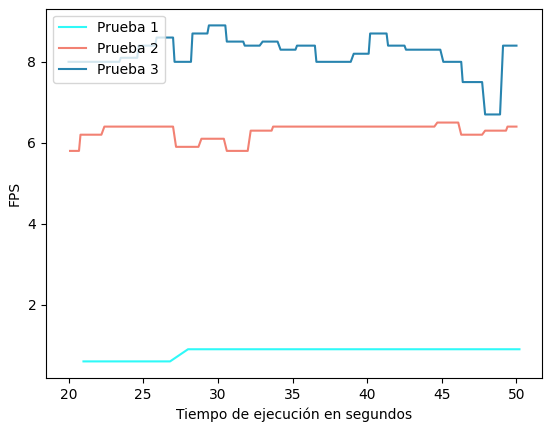
\includegraphics[width=10cm]{figs/dlib_rendimiento.png}
  \end{center}
  \captionsetup{justification=centering}
  \caption{Comparativa de las tres pruebas de rendimiento de dlib.}
  \label{fig:dlib_rendimiento}
\end{figure}

\subsubsection{Prueba de fallos para dlib}

Para comprobar la robustez del algoritmo se evaluó a este en las siguientes condiciones (Figura \ref{fig:dlib_fallos_ejemplos}):

\begin{itemize}
    \item Buenas condiciones lumínicas: 81 fallos.
    \item Malas condiciones lumínicas: 126 fallos.
    \item Rostros parcialmente cubiertos: 188 fallos.
    \item Rostros girados: 183 fallos.
\end{itemize}

\begin{figure}[h!]
  \begin{center}
    \subcapcentertrue
    \subfigure[Buenas condiciones de luz]{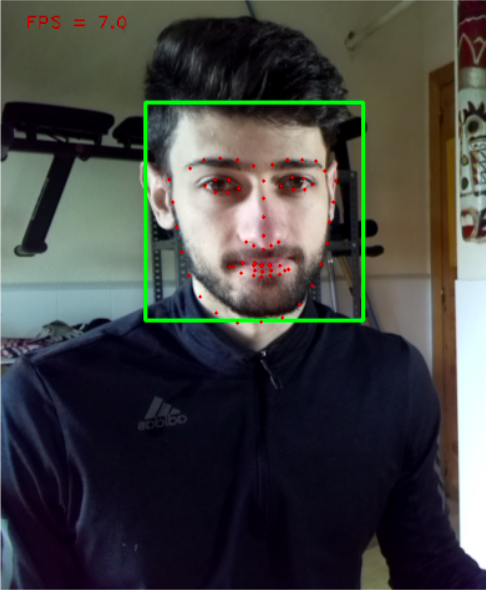
\includegraphics[width=37mm]{figs/dlib_buena_luz.png}}
    \subfigure[Malas condiciones de luz]{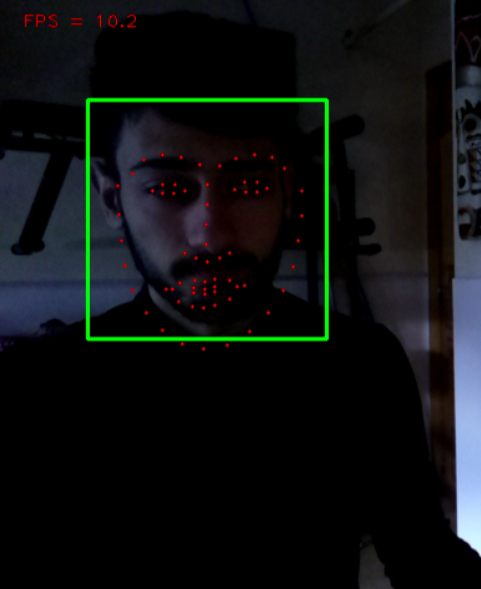
\includegraphics[width=37mm]{figs/dlib_mala_luz.png}}
    \subfigure[Rostros cubiertos]{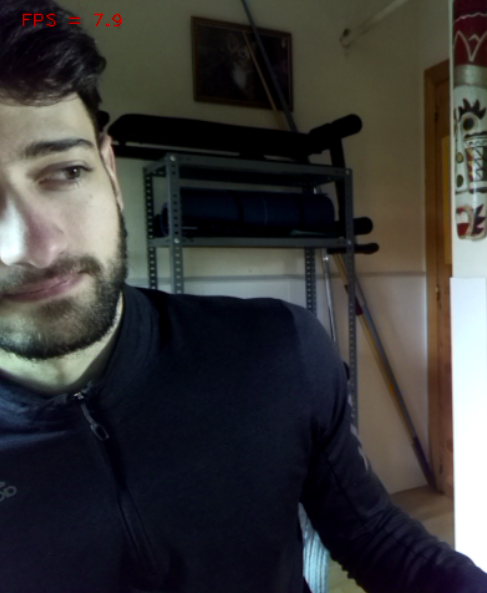
\includegraphics[width=37mm]{figs/dlib_cubiertos.png}}
    \subfigure[Rostros girados]{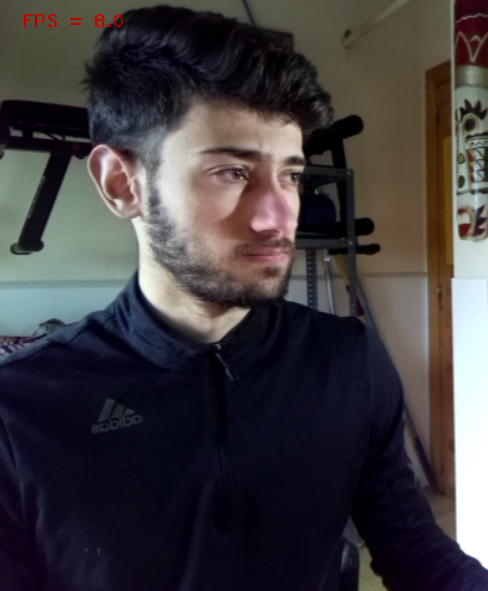
\includegraphics[width=37mm]{figs/dlib_girados.png}}
  \end{center}
\caption{Condiciones en las que se evalúan los fallos de dlib.}
\label{fig:dlib_fallos_ejemplos}
\end{figure}

\subsubsection{Prueba 1 de rendimiento para MediaPipe}
En esta primera prueba se utilizó el algoritmo de la forma general recomendada en el tutorial oficial de MediaPipe. De esta manera, obtuvimos una media de 5.91 fps. Este dato es inferior al resultado final de 8.21 fps de dlib.

\subsubsection{Prueba 2 de rendimiento para MediaPipe}
Llegados a este punto, para mejorar el resultado anterior, dividimos el procesamiento total en \textit{threads} al igual que hicimos con dlib. Dedicamos un \textit{thread} a la lectura de \textit{frames} y el \textit{thread} principal al procesamiento de MediaPipe. De esta manera, aumentamos el rendimiento un 32\%, obteniendo una media de 7.80fps, todavía sin superar el mejor desempeño de dlib.

\subsubsection{Prueba 3 de rendimiento para MediaPipe}
Hasta ahora, estábamos mostrando por pantalla la malla facial detectada, pero esto no será necesario cuando implementemos nuestro sistema de detección de emociones. Por ello, se analizó el rendimiento sin dibujar dicha malla en cada \textit{frame}. De esta manera, el rendimiento subió un 70\% más, llegando así ya a una media de 13.28 fps. Se puede ver una comparativa de las tres pruebas de rendimiento en la Figura \ref{fig:mediapipe_rendimiento}

\begin{figure} [h!]
  \begin{center}
    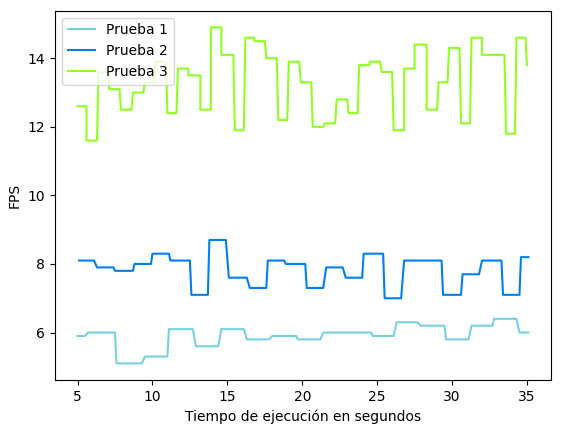
\includegraphics[width=10cm]{figs/mediapipe_rendimiento.png}
  \end{center}
  \captionsetup{justification=centering}
  \caption{Comparativa de las tres pruebas de rendimiento de MediaPipe.}
  \label{fig:mediapipe_rendimiento}
\end{figure}

\subsubsection{Prueba de fallos para MediaPipe}

Para comprobar la robustez del algoritmo se evaluó a este en las siguientes condiciones (Figura \ref{fig:mediapipe_fallos_ejemplos}):

\begin{itemize}
    \item Buenas condiciones lumínicas: 0 fallos.
    \item Malas condiciones lumínicas: 0 fallos.
    \item Rostros parcialmente cubiertos: 103 fallos.
    \item Rostros girados: 0 fallos.
\end{itemize}

\begin{figure}[h!]
  \begin{center}
  \subcapcentertrue
    \subfigure[Buenas condiciones de luz]{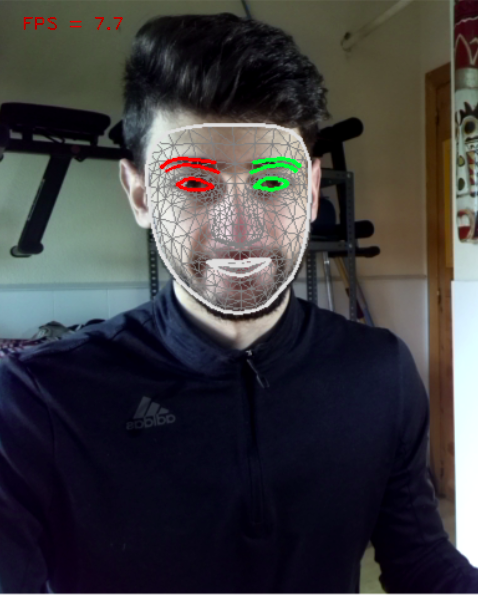
\includegraphics[width=37mm]{figs/mediapipe_buena_luz.png}}
    \subfigure[Malas condiciones de luz]{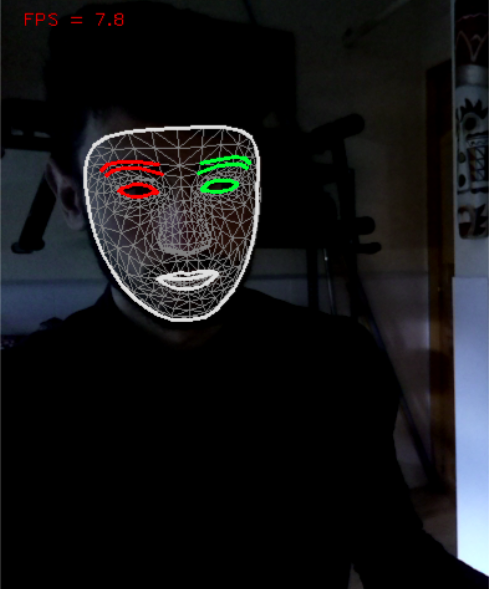
\includegraphics[width=38mm]{figs/mediapipe_mala_luz.png}}
    \subfigure[Rostros cubiertos]{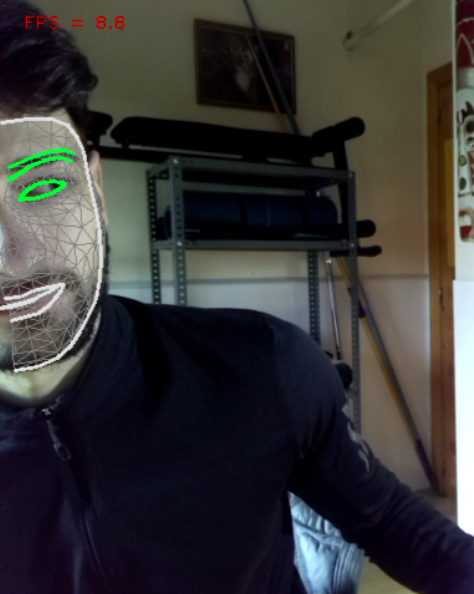
\includegraphics[width=37mm]{figs/mediapipe_cubiertos.png}}
    \subfigure[Rostros girados]{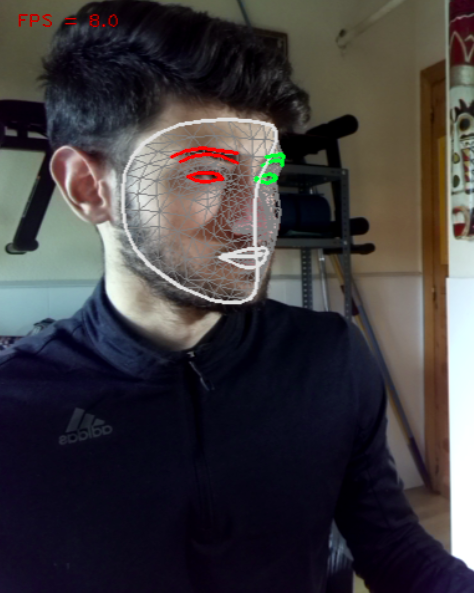
\includegraphics[width=37mm]{figs/mediapipe_girados.png}}
  \end{center}
\caption{Condiciones en las que se evalúan los fallos de MediaPipe.}
\label{fig:mediapipe_fallos_ejemplos}
\end{figure}

Llegados a este punto, podemos concluir afirmando que el algoritmo que mejor rendimiento y precisión nos ofrece es el de MediaPipe. Este ha obtenido un rendimiento de 13.28 fps de media, frente a los 8.21 fps de dlib y OpenCV. Además, este último ha obtenido un total de 578 fallos, frente a los 103 fallos de MediaPipe.

\section{Cantidad de ángulos a utilizar en el dataset}
\label{sec:estudio_cantidad_de_angulos}

El número de ángulos a utilizar de la \textit{malla emocional}, hace referencia a la cantidad de características que posee nuestro dataset. Es por ello, que se debe estudiar cuál es la cantidad óptima de los mismos que mejores resultados nos ofrece a la hora de entrenar los modelos.\\

En primer lugar se realizó un estudio para comprobar qué ángulos de toda la malla son más influyentes en las emociones y, posteriormente, se hizo un estudio de simetría con dichos ángulos, para así comprobar si las emociones se pueden considerar simétricas en ambas mitades de un rostro y entonces únicamente utilizar los ángulos de una sola mitad.

\subsection{Estudio de los ángulos más influyentes en cada emoción}

Tal como se ha comentado anteriormente, realizamos un estudio para escoger los ángulos más influyentes en cada emoción, esto es, los ángulos que más varían cada vez que se producen dichas expresiones faciales. Para realizar esta prueba, partimos de todos los ángulos de la parte derecha del rostro (Figura \ref{fig:emotional_mesh_todos_angulos}), y se calculó la variación que existe en cada uno de ellos y para cada una de las emociones de CK+, desde una posición neutral de la cara hasta la máxima expresión.\\

\begin{figure} [h!]
  \begin{center}
    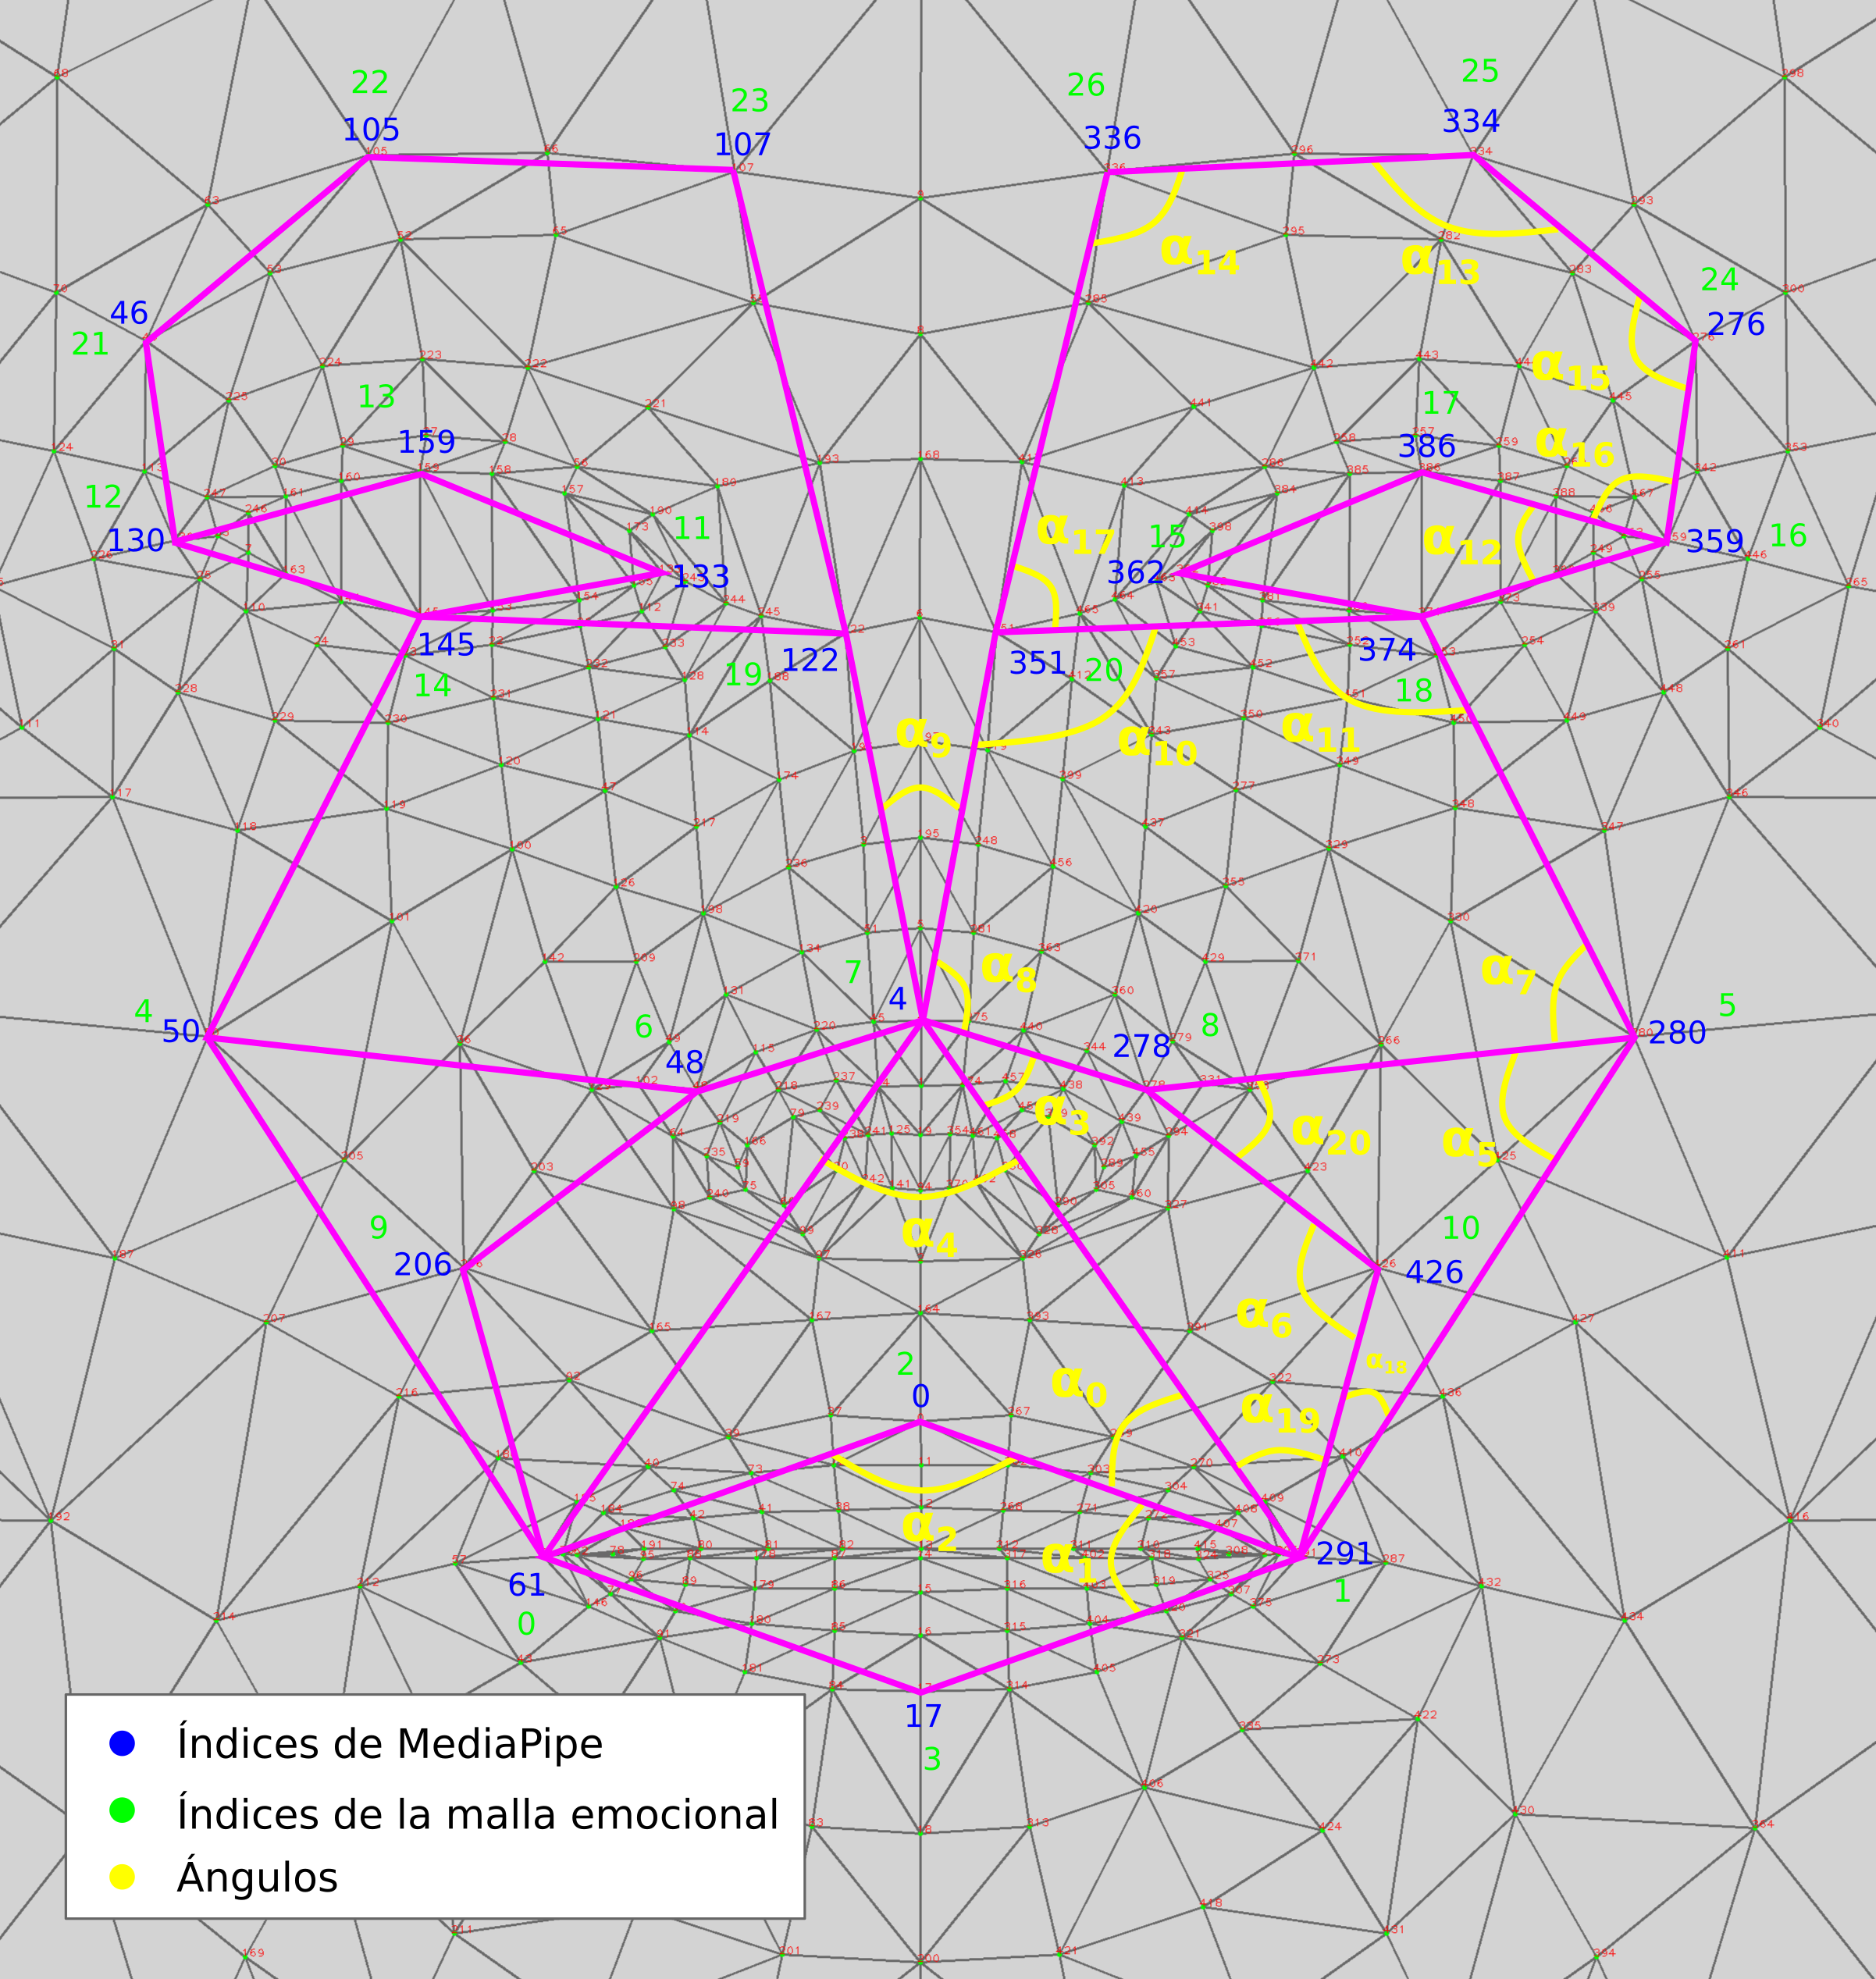
\includegraphics[width=13cm]{figs/emotional_mesh_todos_angulos.png}
  \end{center}
  \captionsetup{justification=centering}
  \caption{Todos los ángulos de la mitad derecha\\
  de la \textit{malla emocional}.}
  \label{fig:emotional_mesh_todos_angulos}
\end{figure}

El método a seguir que nos proporcionó esa variación, fue calcular la diferencia del ángulo en posición neutral respecto a la posición de la máxima expresión, para ello utilizamos el Código \ref{cod:angulos_diferencia}. Este, además de calcular la diferencia, evitó que apareciesen resultados de otros cuadrantes o negativos. Se realizó este cálculo para cada una de las imágenes de CK+ y los resultados fueron las medias calculadas. El resultado del estudio se encuentra en la Figura \ref{fig:estudio_influencia}.\\

\begin{code}[h]
\begin{lstlisting}[language=Python]
def angle_difference(alpha, beta):
    phi = abs(beta-alpha)%360
    if phi > 180:
        return (360 - phi)
    return phi
\end{lstlisting}
\captionsetup{justification=centering}
\caption[Diferencia entre dos ángulos.]{Diferencia entre dos ángulos.}
\label{cod:angulos_diferencia}
\end{code}

Como conclusiones de este estudio, sacamos en claro que los cinco ángulos más influyentes en cada emoción son los mostrados en el Cuadro \ref{cuadro:angulos_5_influyentes} y, que por lo tanto, los ángulos que más varían en total son: 2, 12, 1, 16, 15, 4, 6, 14, 18, 8, 0 y 19.\\

\begin{table}[H]
\begin{center}
\begin{tabular}{|c|c|}
     \hline
    \textbf{Emoción} & \textbf{Ángulos influyentes} \\
    \hline
     Felicidad & 4, 2, 18, 12, 8 \\
     Tristeza & 2, 1, 12, 16, 14 \\
     Sorpresa & 1, 2, 0, 4, 19 \\
     Miedo & 2, 4, 6, 1, 14 \\
     Enfado & 2, 12, 1, 16, 15 \\
     Asco & 12, 16, 2, 15, 1 \\
     Desprecio & 2, 1, 4, 0, 19 \\
     \hline
 \end{tabular}
 \captionsetup{justification=centering}
\caption{Lista de los 5 ángulos más influyentes por cada emoción.}
\label{cuadro:angulos_5_influyentes}
\end{center}
\end{table}

\subsection{Estudio de simetría de las emociones}
Con el afán de descubrir si es posible entrenar a nuestro modelo con sólo ángulos de una mitad del rostro se realizó un estudio de simetría, en el que comprobamos si las emociones se pueden considerar simétricas para ambos lados de la cara. Para ello, partimos de los ángulos obtenidos en el estudio anterior (los más influyentes) y generamos un nuevo mapa que abarca las dos mitades del rostro (Figura \ref{fig:emotional_mesh_2_mitades}).\\

\begin{figure} [h!]
  \begin{center}
    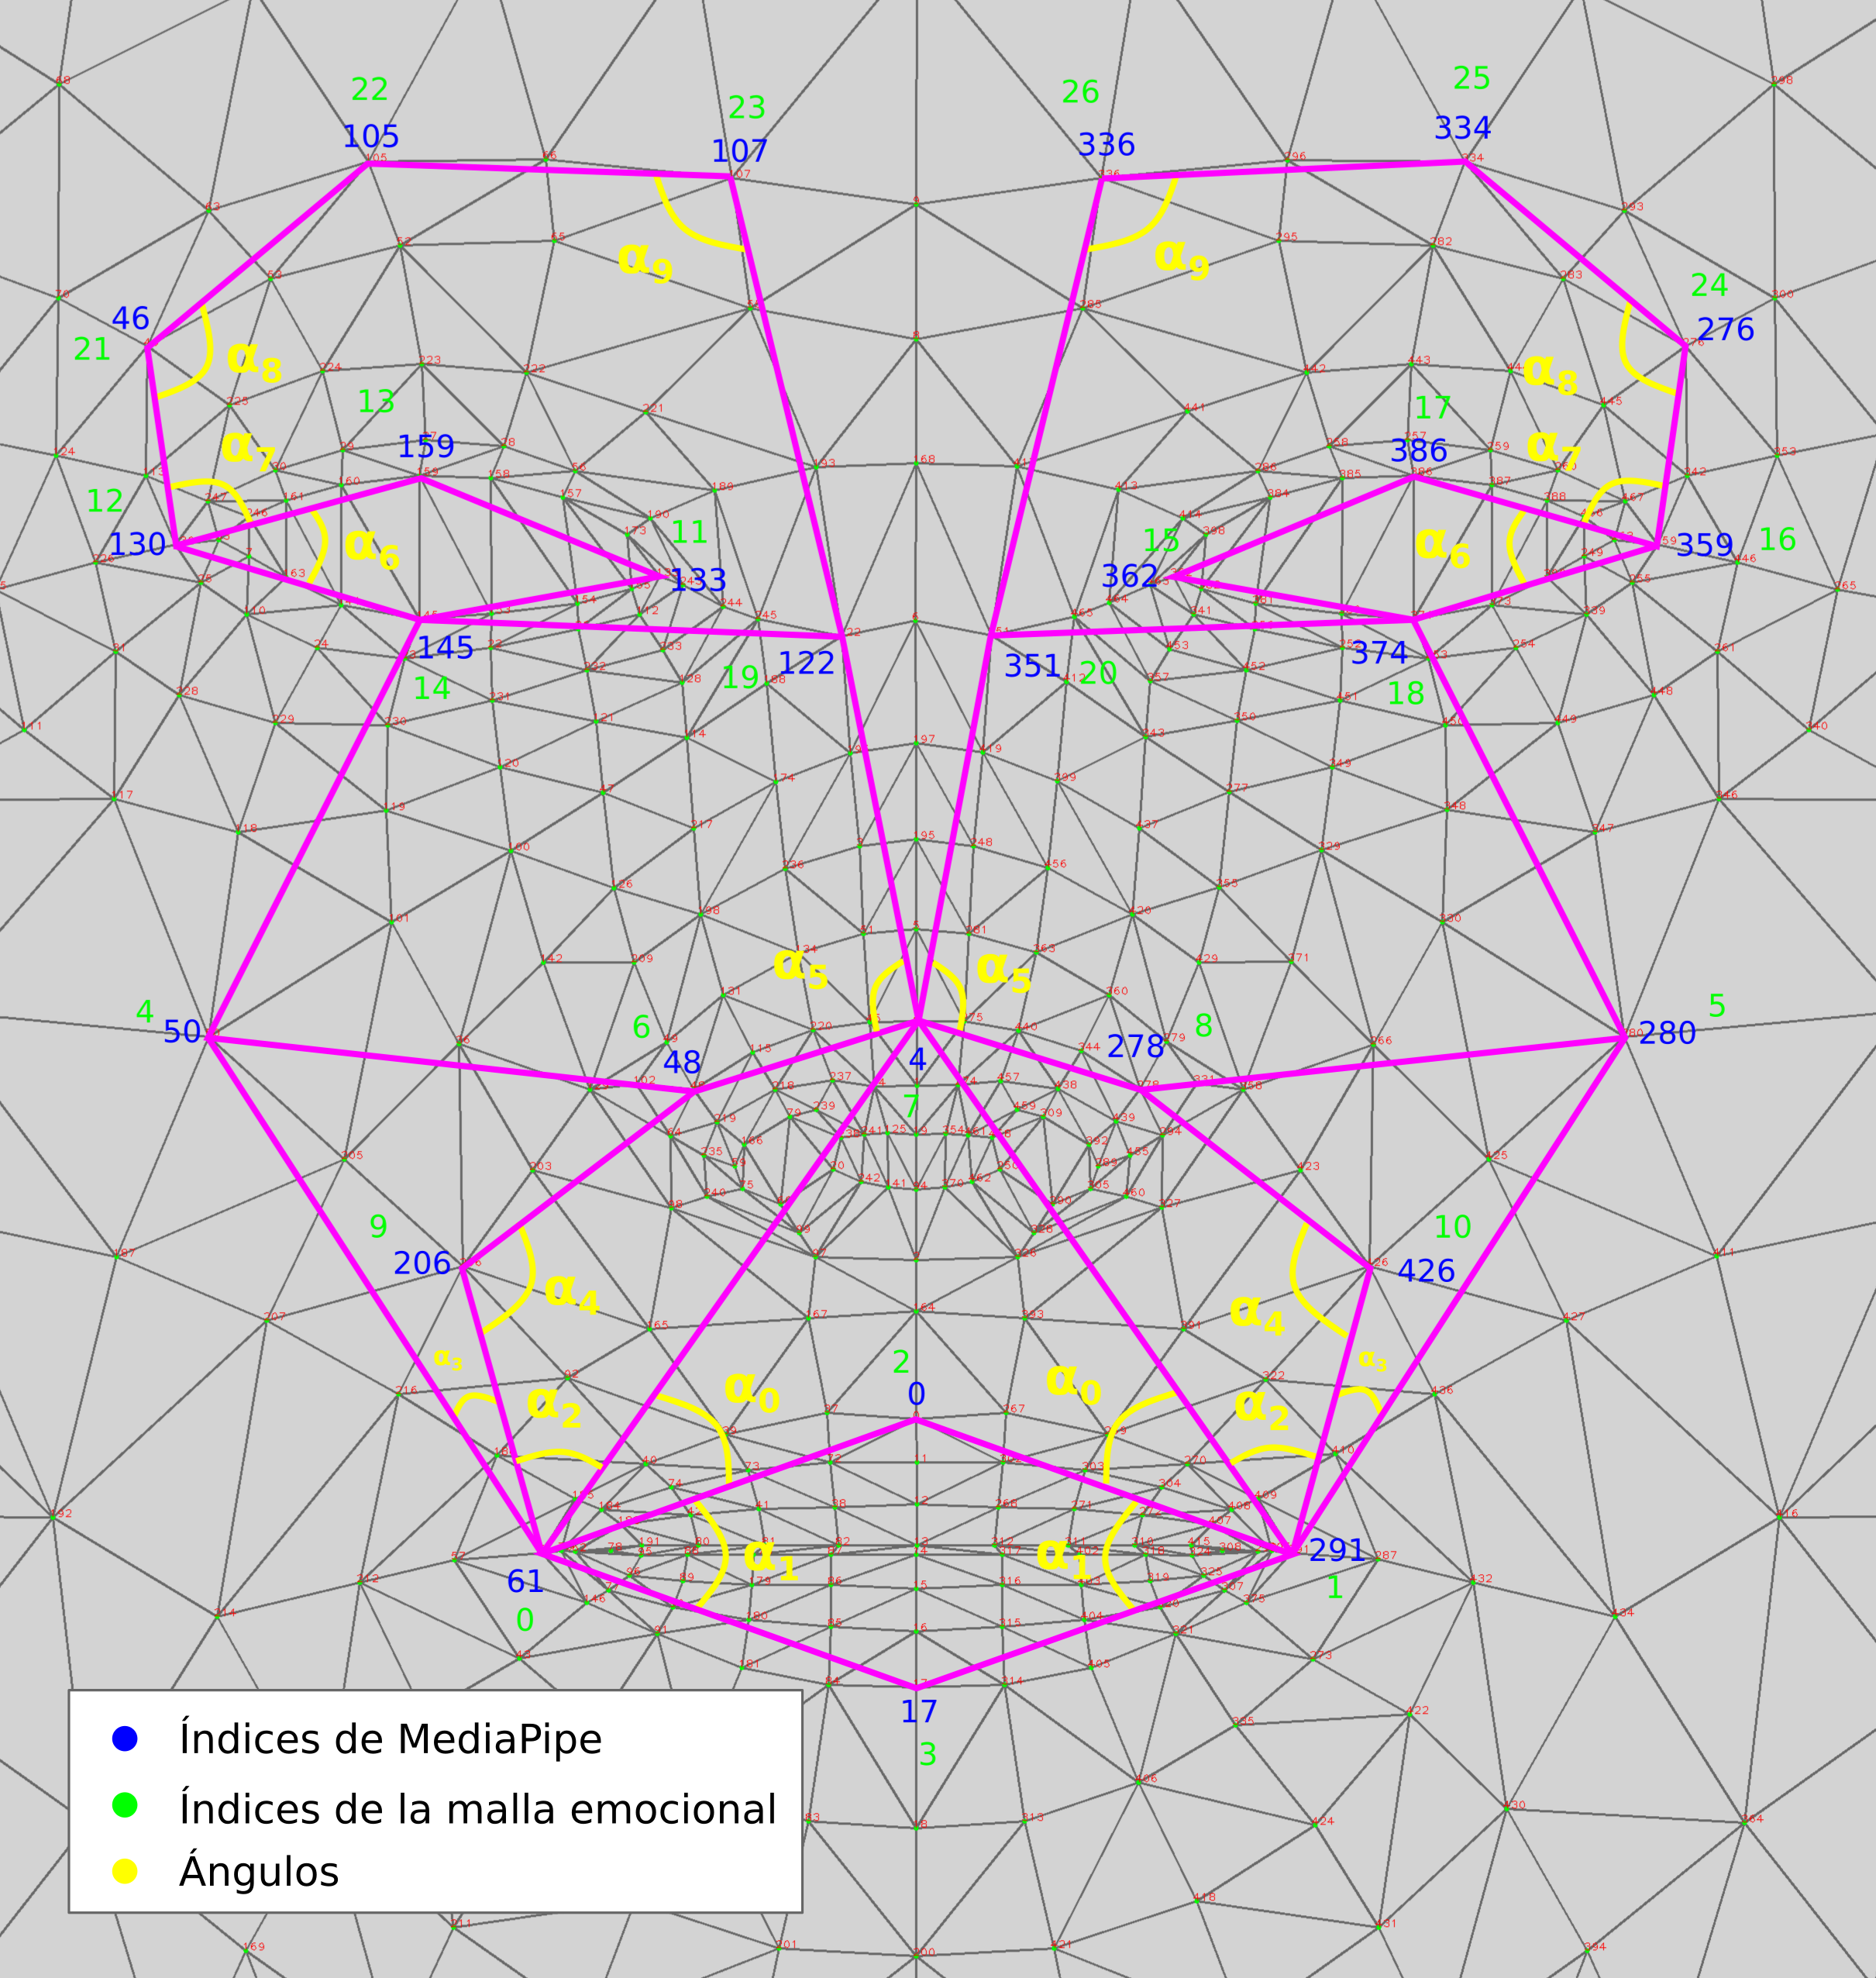
\includegraphics[width=13cm]{figs/emotional_mesh_2_mitades.png}
  \end{center}
  \captionsetup{justification=centering}
  \caption{Mapa de ángulos para realizar el estudio de simetría.}
  \label{fig:emotional_mesh_2_mitades}
\end{figure}

A la hora de estudiar la simetría calculamos la variación que existe entre los ángulos del lado izquierdo y del lado derecho para cada una de las emociones y cada una de las imágenes del dataset CK+. La forma de llevar a cabo este cálculo ha sido la misma que en el estudio anterior (Código \ref{cod:angulos_diferencia}). Los resultados son la media de lo obtenido para todas las imágenes (Figura \ref{fig:estudio_simetría}).\\

Observando los resultados, podemos considerar que las emociones son simétricas, ya que la mayor variación de media entre el lado izquierdo y derecho ha sido de 5 grados, siendo esta una variación mínima. Por lo tanto, conociendo las información de los dos estudios, descartamos todos los ángulos de una mitad de la cara y generamos los dos siguientes datasets:

\begin{itemize}
    \item Base de datos con sólo los ángulos más influyentes de la parte derecha de la \textit{malla emocional}.
    \item Base de datos con todos los ángulos de la parte derecha de la \textit{malla emocional}.
\end{itemize}

En las siguientes secciones se analizó cual de ellos finalmente ofreció mejores resultados en el entrenamiento.

\section{Búsqueda del dataset óptimo para el entrenamiento}
\label{sec:estudio_dataset_optimo}

Se realizó un estudio en búsqueda del dataset que mejores resultados nos ofrecía a la hora de realizar el entrenamiento. Para ello se probó con los dos datasets generados en la sección anterior a raíz de los estudios de influencia (Sección \ref{fig:estudio_influencia}) y de simetría (Sección \ref{fig:estudio_simetría}). De aquí en adelante se utilizan los siguientes nombres para identificar a cada uno de los datasets:

\begin{itemize}
    \item \textbf{\textit{dataset1}}: base de datos con sólo los ángulos más influyentes de la parte derecha de la \textit{malla emocional}.
    \item \textbf{\textit{dataset2}}: base de datos con todos los ángulos de la parte derecha de la \textit{malla emocional}.
\end{itemize}

Ambos han sido entrenados por los clasificadores KNN, SVM y MLP y, además, con el \textit{dataset2} se ha utilizado PCA para reducir el número de características. Se desea comprobar si ofrece más rendimiento el \textit{dataset1} habiendo reducido los ángulos de forma manual (sólo contiene los más influyentes de cada emoción) o el \textit{dataset2} reduciéndolos usando PCA.

\subsubsection{Entrenamiento usando el \textit{dataset1}}

Los parámetros óptimos de los tres clasificadores, tras realizar su búsqueda usando validación cruzada KFoldStratified de 4 \textit{pliegues}, se encuentran en el Cuadro \ref{cuadro:parametros_dataset1}. Para KNN se ha probado con valores de k impares entre 1 y 13 incluidos, para SVM con valores de C entre 1 y 999 (saltos de 10 en 10) y para MLP se ha probado con 1 capa oculta de neuronas entre 5 y 24 incluidos, no ha sido necesario añadir más capas.\\

\begin{table}[H]
\begin{center}
\begin{tabular}{|c|c|}
     \hline
    \textbf{Clasificador} & \textbf{Parámetros} \\
    \hline
     KNN & \verb|k = 11| \\
     SVM & \verb|C = 11| \\
     MLP & \verb|hidden_layer_sizes = (19)|\\
     \hline
 \end{tabular}
 \captionsetup{justification=centering}
\caption{Parámetros óptimos para cada uno de los clasificadores\\
entrenando con el \textit{dataset1}.}
\label{cuadro:parametros_dataset1}
\end{center}
\end{table}

Los resultados obtenidos en el entrenamiento para el \textit{dataset1} usando los parámetros óptimos, se encuentran en el Cuadro \ref{cuadro:resultados_dataset1}. Estos han sido calculados también mediante validación cruzada KFoldStratified de 4 \textit{pliegues}, y se muestra la media de todas las iteraciones.\\

\begin{table}[H]
\begin{center}
\begin{tabular}{|c|c|c|c|c|}
     \hline
    \textbf{Clasificador} & \textbf{Accuracy} & \textbf{Precision} & \textbf{Recall} & \textbf{F1-score}\\
    \hline
     KNN & 0.82 & 0.76 & 0.74 & 0.74\\
     SVM & 0.84 & 0.79 & 0.78 & 0.77\\
     MLP & 0.82 & 0.78 & 0.78 & 0.77\\
     \hline
 \end{tabular}
 \captionsetup{justification=centering}
\caption{Resultados de precisión de los clasificadores\\
usando el \textit{dataset1}.}
\label{cuadro:resultados_dataset1}
\end{center}
\end{table}

\subsubsection{Entrenamiento usando el \textit{dataset2}}

El valor óptimo de características a mantener por PCA y los parámetros para cada clasificador tras realizar su búsqueda usando validación cruzada KFoldStratified de 4 \textit{pliegues}, se encuentran en el Cuadro \ref{cuadro:parametros_dataset2}. Para hacer la reducción con PCA se ha probado con un número de componentes entre 2 y 20 incluidos, para KNN se ha probado con valores de k impares entre 1 y 13 incluidos, para SVM con valores de C entre 1 y 999 (saltos de 10 en 10) y para MLP se ha probado con 1 capa oculta de neuronas entre 5 y 24 incluidos, no ha sido necesario añadir más capas.\\

\begin{table}[H]
\begin{center}
\begin{tabular}{|c|c|}
     \hline
    \textbf{Clasificador y PCA} & \textbf{Parámetros} \\
    \hline
     KNN y PCA & \verb|k = 11|, \verb|n_components = 17|\\
     SVM y PCA & \verb|C = 11|, \verb|n_components = 7|\\
     MLP y PCA & \verb|hidden_layer_sizes = (12)|, \verb|n_components = 11|\\
     \hline
 \end{tabular}
 \captionsetup{justification=centering}
\caption{Parámetros óptimos para cada uno de los clasificadores\\
entrenando con el \textit{dataset2}.}
\label{cuadro:parametros_dataset2}
\end{center}
\end{table}

Los resultados obtenidos en el entrenamiento para el \textit{dataset2} usando los parámetros óptimos, se encuentran en el Cuadro \ref{cuadro:resultados_dataset2}. Estos resultados de precisión han sido calculados también mediante validación cruzada KFoldStratified de 4 \textit{pliegues}, y se muestra la media de todas las iteraciones.\\

\begin{table}[H]
\begin{center}
\begin{tabular}{|c|c|c|c|c|}
     \hline
    \textbf{Clasificador} & \textbf{Accuracy} & \textbf{Precision} & \textbf{Recall} & \textbf{F1-score}\\
    \hline
     KNN & 0.83 & 0.79 & 0.75 & 0.75\\
     SVM & 0.84 & 0.80 & 0.77 & 0.78\\
     MLP & 0.84 & 0.81 & 0.80 & 0.80\\
     \hline
 \end{tabular}
 \captionsetup{justification=centering}
\caption{Resultados de precisión de los clasificadores\\
usando el \textit{dataset2}.}
\label{cuadro:resultados_dataset2}
\end{center}
\end{table}

\subsubsection{Conclusiones}
Los resultados obtenidos para cada uno de los datasets son bastante similares, aunque un poco superiores para el \textit{dataset2}, sobre todo si observamos \textit{Precision}, \textit{Recall} y \textit{F1-score}. En cuanto a los resultados obtenidos por cada clasificador, también son muy similares y sería muy complicado decantarse por uno sólo.\\

Sin embargo, en general no son resultados demasiado buenos y la herramienta robótica construida a partir de estos modelos no sería muy robusta. Sobre todo si observamos los resultados de cada una de las clases por separado, por ejemplo los arrojados por SVM usando el \textit{dataset2} (Cuadro \ref{cuadro:resultados_SVM}). En dichos resultados, podemos observar que clases como ---por ejemplo--- la de \textit{Desprecio} o la de \textit{Enfado} han obtenido puntuaciones malas, incluso por debajo del 50\% en algún caso. Por lo tanto, esto nos lleva a pensar que nuestro sistema no va a dar buen rendimiento a la hora de detectar todas las emociones, aunque de media si que tenga una puntuación aceptable.\\

\begin{table}[h!]
\begin{minipage}{0.48\linewidth}
\centering
\begin{adjustbox}{max width=\textwidth}
\begin{tabular}{|c|c|c|c|}
\hline
\textbf{Clase} & \textbf{Precision} & \textbf{Recall} & \textbf{F1-score}\\
\hline
     Enfado & 0.67 & 0.50 & 0.57\\
     Desprecio & 0.67 & 0.50 & 0.57\\
     Asco & 0.76 & 0.87 & 0.81\\
     Miedo & 0.67 & 1.00 & 0.80\\
     Felicidad & 0.94 & 0.94 & 0.94\\
     Tristeza & 0.83 & 0.71 & 0.77\\
     Sorpresa & 0.95 & 0.95 & 0.95\\
\hline
\end{tabular}
\end{adjustbox}
\vspace{0.5cm}

\begin{adjustbox}{max width=\textwidth}
\begin{tabular}{|c|c|c|c|}
\hline
\textbf{Clase} & \textbf{Precision} & \textbf{Recall} & \textbf{F1-score}\\
\hline
     Enfado & 0.75 & 0.82 & 0.78\\
     Desprecio & 0.67 & 0.80 & 0.73\\
     Asco & 0.82 & 0.93 & 0.87\\
     Miedo & 0.80 & 0.67 & 0.73\\
     Felicidad & 0.94 & 0.94 & 0.94\\
     Tristeza & 1.00 & 0.57 & 0.73\\
     Sorpresa & 0.95 & 0.95 & 0.95\\
\hline
\end{tabular}
\end{adjustbox}
\end{minipage}\hfill
\begin{minipage}{0.48\linewidth}
\centering
\begin{adjustbox}{max width=\textwidth}
\begin{tabular}{|c|c|c|c|}
\hline
\textbf{Clase} & \textbf{Precision} & \textbf{Recall} & \textbf{F1-score}\\
\hline
     Enfado & 0.71 & 0.45 & 0.56\\
     Desprecio & 0.57 & 0.80 & 0.67\\
     Asco & 0.76 & 0.93 & 0.84\\
     Miedo & 1.00 & 0.71 & 0.83\\
     Felicidad & 0.85 & 1.00 & 0.92\\
     Tristeza & 0.83 & 0.71 & 0.77\\
     Sorpresa & 1.00 & 0.95 & 0.98\\
\hline
\end{tabular}
\end{adjustbox}
\vspace{0.5cm}

\begin{adjustbox}{max width=\textwidth}
\begin{tabular}{|c|c|c|c|}
\hline
\textbf{Clase} & \textbf{Precision} & \textbf{Recall} & \textbf{F1-score}\\
\hline
     Enfado & 0.67 & 0.55 & 0.60\\
     Desprecio & 0.50 & 0.25 & 0.33\\
     Asco & 0.67 & 0.80 & 0.73\\
     Miedo & 1.00 & 0.67 & 0.80\\
     Felicidad & 1.00 & 1.00 & 1.00\\
     Tristeza & 0.50 & 0.71 & 0.59\\
     Sorpresa & 1.00 & 1.00 & 1.00\\
\hline
\end{tabular}
\end{adjustbox}
\end{minipage}
\captionsetup{justification=centering}
\caption{Resultados del entrenamiento con SVM en cada una\\
de las 4 iteraciones de KFoldStratified usando el \textit{dataset2}.}
\label{cuadro:resultados_SVM}
\end{table}

Esta mala clasificación de algunas emociones se debe a la gran similitud que existe entre varias. Esto provoca que geométricamente sean prácticamente indiferenciables, y por lo tanto, es complicado que los algoritmos sepan clasificarlas correctamente. Si observamos el estudio de ángulos influyentes en cada emoción (Figura \ref{fig:estudio_influencia}) (Cuadro \ref{cuadro:angulos_5_influyentes}), podemos ver que ---por ejemplo--- las emociones \textit{sorpresa} y \textit{desprecio} poseen exactamente los mismos 5 ángulos influyentes, o las emociones \textit{enfado} y \textit{asco} que también poseen los mismos 5. Esto dificulta muchísimo la tarea de clasificación.\\

Por lo tanto, se propuso eliminar las emociones que estén interceptando con otras y, de esta manera, aumentar la robustez de nuestra futura herramienta consiguiendo mayor precisión en nuestro modelo. Las emociones que se eligieron son las siguientes: \textit{felicidad}, \textit{tristeza}, \textit{sorpresa} y \textit{enfado}. Son las 4 emociones simples más generales y, además, se diferencian geométricamente unas de otras. Sabiendo esto, el dataset ganador y, por lo tanto el que es usado para entrenar nuestro sistema final, es el \textit{dataset2} con las emociones de \textit{felicidad}, \textit{tristeza}, \textit{sorpresa} y \textit{enfado}.

\begin{figure}[h!]
  \begin{center}
    \subcapcentertrue
    \subfigure[Felicidad]{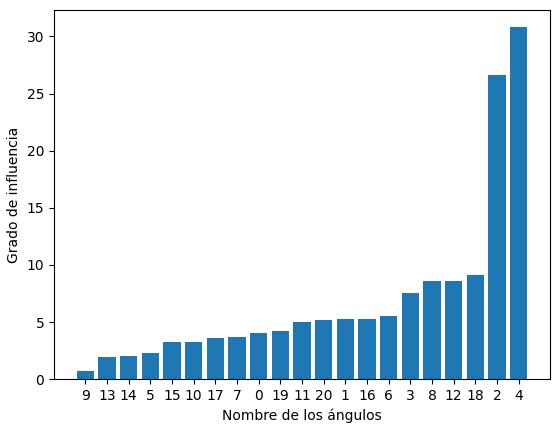
\includegraphics[width=60mm]{figs/diferencia_happy.png}}
    \subfigure[Tristeza]{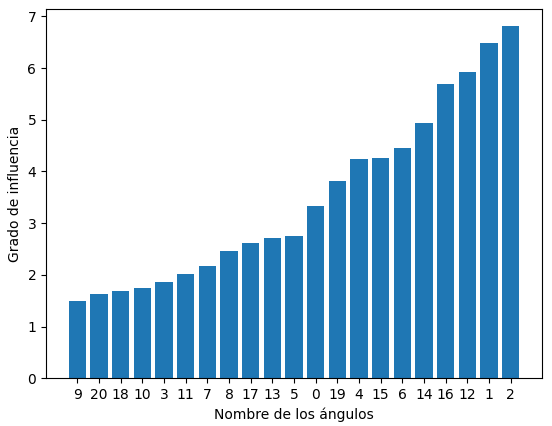
\includegraphics[width=60mm]{figs/diferencia_sadness.png}}
    \subfigure[Sorpresa]{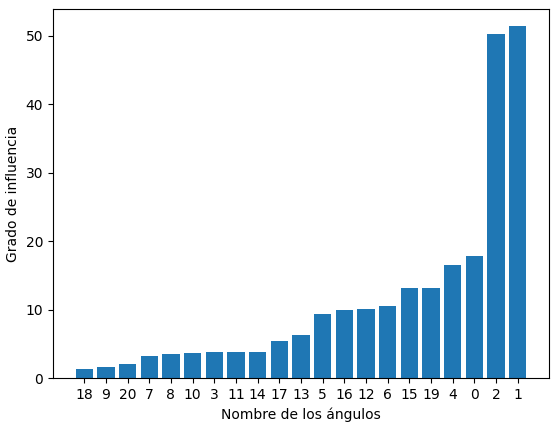
\includegraphics[width=60mm]{figs/diferencia_surprise.png}}
    \subfigure[Miedo]{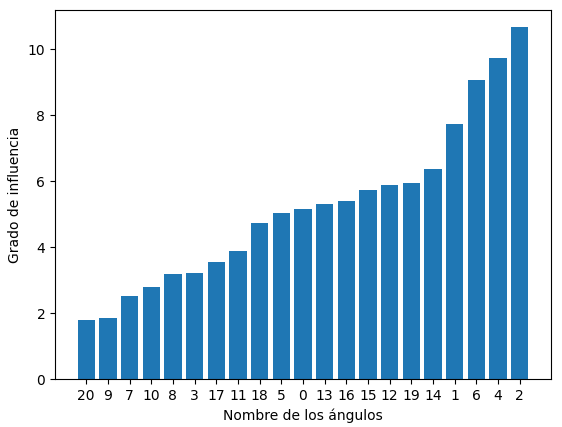
\includegraphics[width=60mm]{figs/diferencia_fear.png}}
    \subfigure[Enfado]{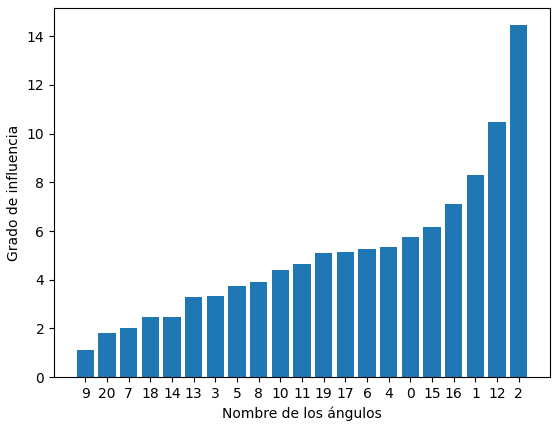
\includegraphics[width=60mm]{figs/diferencia_anger.png}}
    \subfigure[Asco]{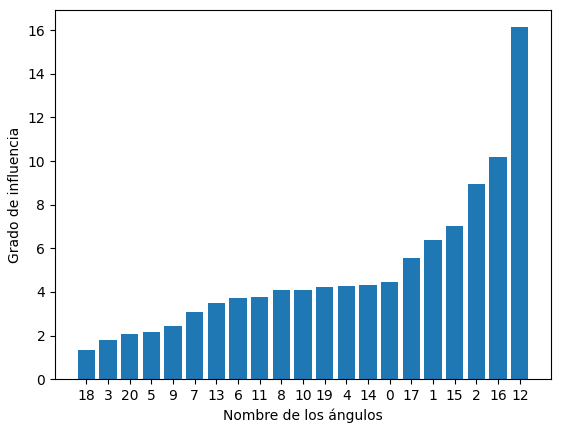
\includegraphics[width=60mm]{figs/diferencia_disgust.png}}
    \subfigure[Desprecio]{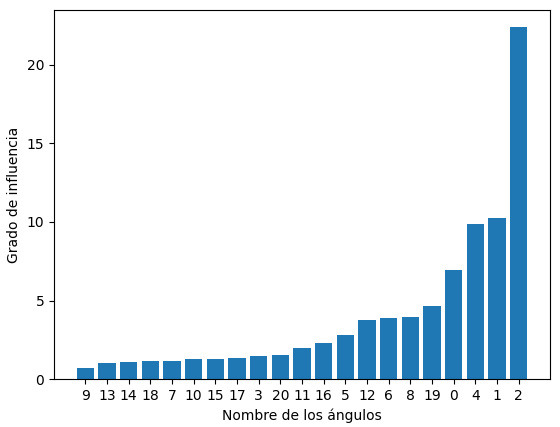
\includegraphics[width=60mm]{figs/diferencia_contempt.png}}
  \end{center}
\captionsetup{justification=centering}
\caption{Estudio de los ángulos más influyentes para cada emoción.}
\label{fig:estudio_influencia}
\end{figure}

\begin{figure}[h!]
  \begin{center}
    \subcapcentertrue
    \subfigure[Felicidad]{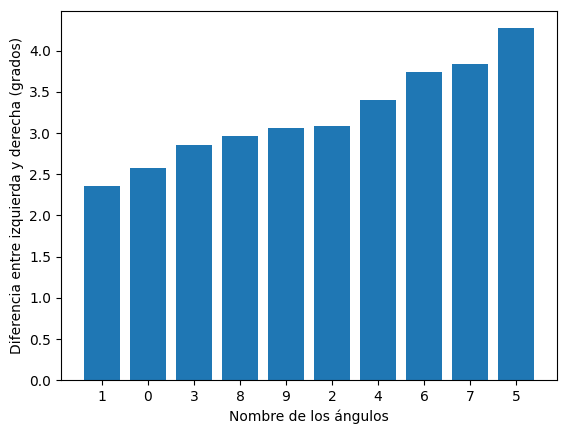
\includegraphics[width=60mm]{figs/diferencia_izq_der_happy.png}}
    \subfigure[Tristeza]{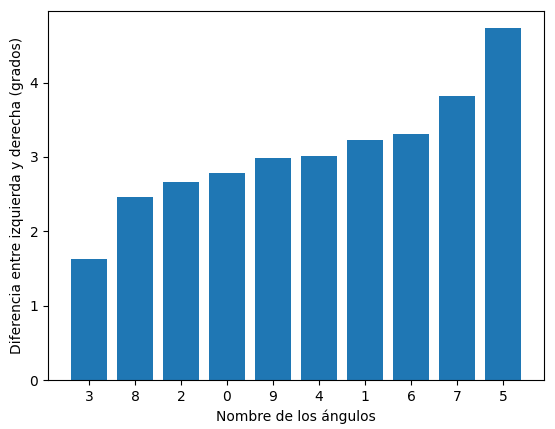
\includegraphics[width=60mm]{figs/diferencia_izq_der_sadness.png}}
    \subfigure[Sorpresa]{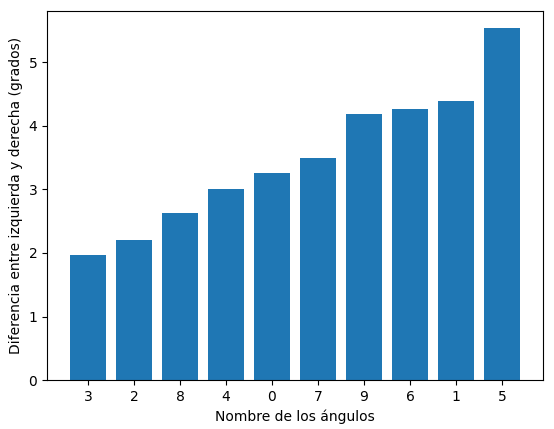
\includegraphics[width=60mm]{figs/diferencia_izq_der_surprise.png}}
    \subfigure[Miedo]{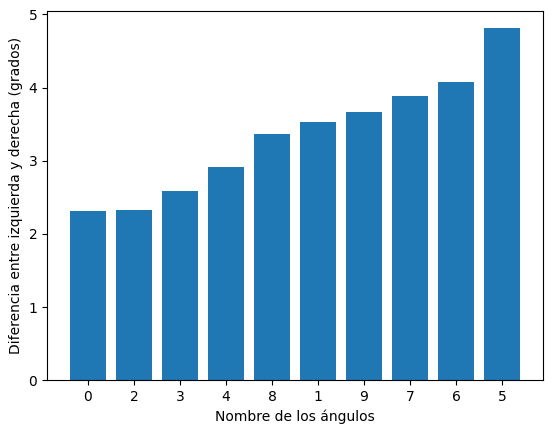
\includegraphics[width=60mm]{figs/diferencia_izq_der_fear.png}}
    \subfigure[Enfado]{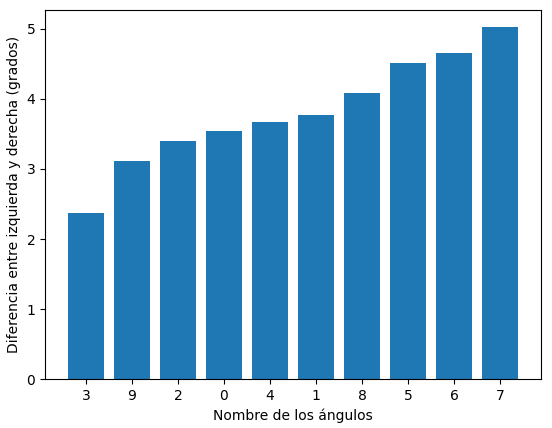
\includegraphics[width=60mm]{figs/diferencia_izq_der_anger.png}}
    \subfigure[Asco]{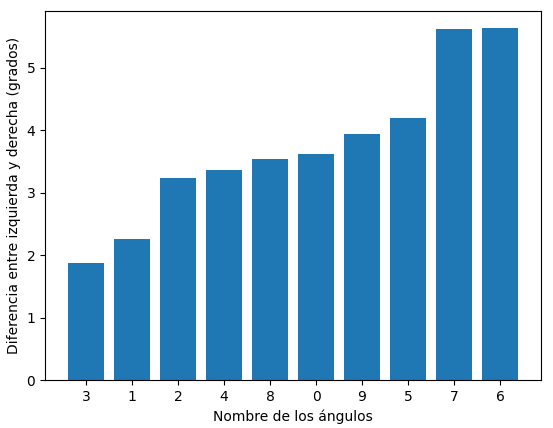
\includegraphics[width=60mm]{figs/diferencia_izq_der_disgust.png}}
    \subfigure[Desprecio]{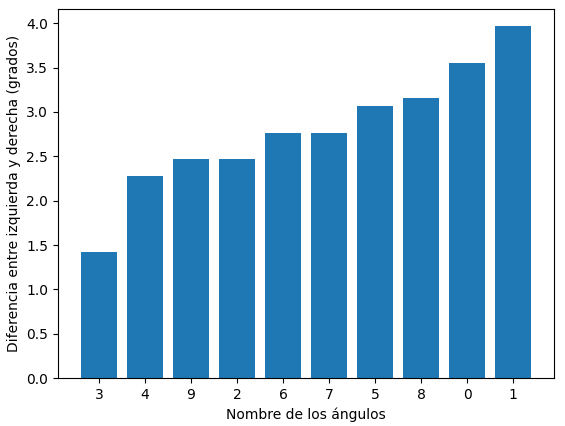
\includegraphics[width=60mm]{figs/diferencia_izq_der_contempt.png}}
  \end{center}
\captionsetup{justification=centering}
\caption{Estudio de simetría para cada una de las emociones.}
\label{fig:estudio_simetría}
\end{figure}